\documentclass[9pt,a4paper]{article}
\usepackage{amsfonts,amsmath,amsthm,amssymb,graphicx,graphics}
\usepackage{setspace,wrapfig,colortbl,indentfirst,caption,multirow}
\usepackage[utf8x]{inputenc}
\renewcommand\figurename{Figura}
\newtheorem{definitie}{Definiție}

\title{\bf Laborator 6}
\author{Sîrbu Matei-Dan}
\date{19 noiembrie 2020}

\begin{document}
\maketitle

\section*{Exercițiul 1}
\subsection*{Breviar teoretic}

\begin{doublespace}
    Printre cele mai utilizate structuri de date sunt listele, două tipuri speciale de liste: stiva și coada, și nu în ultimul rând o structură de storcare asociativă numită \textit{map}.

    O \textit{listă} reprezintă o secvență de zero (lista vidă) sau mai multe elemente de un anumit tip:
    $$a_1, a_2, \dots, a_n$$
    unde $n \geq 0$ și este numit lungimea listei (n = 0 listă vidă) iar $a_i$ este elementul din listă de pe poziția $i$ ($1 \leq i \leq n$). Cele mai importante operații cu o listă sunt

    \begin{itemize}
        \item \textit{INSERT(x, p, L)}. Inserarea adaugă în lista $L$ elementul $x$ la poziția $p$, deplasând la dreapta toate elementele care se aflau pe pozițiile $p, \dots, n$.
        \item \textit{LOCATE(x, L)}. Returnează poziția elementului $x$ în lista L. Dacă $x$ apare de mai multe ori poziția primei apariții este returnată.
        \item \textit{RETRIEVE(p, L)}. Returnează elementul aflat pe poziția $p$ în lista L.
        \item \textit{DELETE(p, L)}. Șterge elementul de pe poziția $p$ din lista $L$ iar elementele de pe pozițiile $p+1, \dots, n$ sunt mutate cu o poziție la stânga.
        \item \textit{NEXT(p, L)} și \textit{PREVIOUS(p, L)} returnează poziția următoare respectiv anterioară din lista $L$.
    \end{itemize}
\end{doublespace}

\newpage

\section*{Exercițiul 2}
\begin{definitie}
    Variabila aleatoare $X$ urmează \textbf{legea normală (Gauss-Laplace)} (X are repartiție normală) cu parametrii $m$ și $\sigma\ (m \in \mathbb{R}, \sigma > 0)$ dacă densitatea sa de probabilitate (repartiție) este funcția
    \begin{equation}
        f(x;m;\sigma) = \frac{1}{\sigma \sqrt{2 \pi}} \mathrm{e}^{-\frac{(x-m)^2}{2\sigma^2}}
        \label{def:gauss}
    \end{equation}
\end{definitie}

O variabilă aleatoare cu repartiție normală cu parametrii $m$ și $\sigma$ se notează cu $N(m,\sigma^2)$.

Funcția $f$ de mai sus se numește \textit{densitatea de repartiție normală} sau \textit{gaussiană}. Observăm că $f$ este o densitate de probabilitate, deoarece $f(x) > 0, \forall x \in \mathbb{R}$ și $\int_{-\infty}^{\infty} f(x)dx = 1$. Într-adevăr, pentru a verifica ultima relație, în integrala de mai sus facem schimbarea de variabilă $\frac{x-m}{\sigma\sqrt{2}}=y$. Rezultă că $dx = \sigma\sqrt{2} dy$. Dacă $x \rightarrow -\infty$ atunci $y \rightarrow -\infty$, iar dacă $x \rightarrow \infty$ atunci $y \rightarrow \infty$. Obținem astfel
$$\int_{-\infty}^{\infty}f(x)dx = \frac{1}{\sqrt{\pi}}\int_{-\infty}^{\infty}\mathrm{e}^{-y^2}dy = \frac{2}{\sqrt{\pi}}\int_0^{\infty}\mathrm{e}^{-y^2}dy = 1.$$
Am folosit mai sus integrala lui Euler-Poisson $\int_0^\infty \mathrm{e}^{-y^2} dy = \sqrt{\pi}/2$.

\begin{wrapfigure}{R}{0.4\textwidth}
    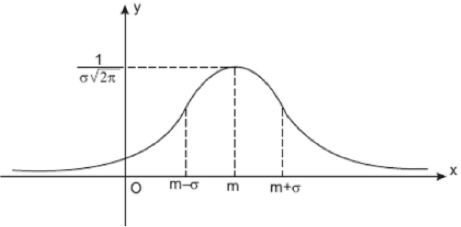
\includegraphics[width=0.4\textwidth]{func_plot.png}
    \caption{Clopotul lui Gauss}
    \label{fig:gauss}
\end{wrapfigure}


Graficul funcției $f$ are formă de clopot (vezi figura \ref{fig:gauss}). Dreapta de ecuație $x = m$ este axă de simetrie pentru acest grafic, iar pentru $x = m$ se obține valoarea maximă a funcției $f$, și anume $\frac{1}{\sigma\sqrt{2\pi}}$. Punctele $x = m - \sigma$ și $x = m + \sigma$ sunt puncte de inflexiune.

\section*{Exercițiul 3}

\begin{tabular}{|c|>{\columncolor[rgb]{0.42,0.84,0.55}}l|>{\columncolor[rgb]{0.58,0.69,0.83}}l|}
    \hline
    \multirow{5}{*}{\bf Valori} & Încredere în sine & Onestitate  \\
                                & Autonomie         & Integritate \\
                                & Independență & Diversitate \\
                                & Spirit antreprenorial & Responsabilitate \\
                                & Diversitate & Munca în echipă \\
    \hline
    \multirow{12}{*}{\bf Caracteristici} & & Sociabil \\
                                & & Încrezător \\
                                & Comfortabil cu schimbările & Optimist \\
                                & Cinic & Orientat spre realizări \\
                                & Pragmatic & Cooperant \\
                                & Flexibil & Educat \\
                                & Multifuncțional & Tehnologizat \\
                                & Creativ & Conștiență socială (socially aware) \\
                                & Autonom & Altruist \\
                                & Țeluri specifice & Multifuncțional \\
                                & & Practic \\
                                & & Team worker \\
    \hline
    \multirow{5}{2cm}{\bf Preferințe la locul de muncă} & Concentrat pe carieră & Muncă semnificativă \\
                                & Echilibru viața profesională - & Job flexibil \\
                                & viața personală & Feedback/Mentoring \\
                                & Lipsa siguranței & Concentrat pe carieră \\
                                & Abordarea informală & \\
    \hline
\end{tabular}

\end{document}